\subsection{Initialization}
\label{sec:genetic_programming:initialization}
  As with other evolutionary algorithms, the algorithm starts by generating a
  population of random individuals.
  
  There are many ways to generate random individuals, but a very common (and
  simple) method is the \emph{grow 
  method}~\autocite{kozaGeneticProgrammingProgramming1992a}.
  In this method, a maximum height is defined, and the algorithm then creates a
  random tree with a given minimum height and a maximum height.

  \begin{remark}
    A tree with a height of 0 is a tree with only one node, the root.
  \end{remark}

  The grow method then proceeds to recursively generate the trees with random
  nodes until a terminal node is selected or the maximum height is reached.
  This method is shown in \vref{alg:genetic_programming:initialization:grow}.

  \begin{algorithm}[ht!]
    \begin{algorithmic}[1]
      \Require \(l \in \mathbb{N}\), \(h \in \mathbb{N}\)
      \Require \(l \leq h\)
      \Require a random integer \(n\) such that \(l \leq n \leq h\)
      \Require \(\mathbf{t}\) and \(\mathbf{f}\) are the sets of terminal and 
        function nodes respectively, where \(\mathbf{t} \neq \emptyset\) and
        \(\mathbf{f} \neq \emptyset\)
      \Ensure a random tree with a height between \(l\) and \(h\)
      \Function{\(\mathrm{grow}\)}{$\mathbf{t}$, $\mathbf{f}$, $d$}
        \State \(c \gets \emptyset\)
        \If{
          \(d = n\ 
            \lor\ \left(
              d \geq l\ 
              \land\ \mathrm{random}() 
                < \mathlarger{\frac{|\mathrm{t}|}{|\mathrm{t}| + |\mathrm{f}|}}
            \right)\)
        }
          \State \Return a random node from \(\mathbf{t}\)
        \Else
          \State \(f \gets\) a random node from \(\mathbf{f}\)
          \For{\(i\) \textbf{in} \(1 \dots \mathrm{arity}(f)\)}
            \State \(c_i \gets 
              \Call{\(\mathrm{grow}\)}{\mathbf{t},\, \mathbf{f},\, d + 1}\)
            \State \(c \gets c \cup \{c_i\}\)
          \EndFor
          \State \Return a tree with root \(f\) and children \(c\)
        \EndIf
      \EndFunction
    \end{algorithmic}
    \caption{The grow method for generating random trees}
    \label{alg:genetic_programming:initialization:grow}
  \end{algorithm}

  With this method, the algorithm can generate trees where the size of the 
  longest path from the root to a leaf is a number \(n \in [l, h]\).

  Now that the algorithm can generate random trees, it can generate a random
  population of trees by generating a random tree for each individual in the
  population.
  Assuming a population size of \(p = 4\), a maximum height of \(h = 3\), a
  minimum height of \(l = 1\), and the primitives set defined in the previous
  section, the algorithm could generate the population: 
  \(
    \mathbf{P} = \{\mathbf{I}_1,\,\mathbf{I}_2,\,\mathbf{I}_3,\,\mathbf{I}_4\} 
      = \left\{
        \frac{3}{\sin(2)} \times 5^3,\,
        7 - (5 + \sin(x)),\,
        7 + 2,\,
        5x^2
      \right\}
  \), as shown in \vref{fig:genetic_programming:initialization:population}.

  \begin{figure}[ht!]
    \centering
    \begin{subfigure}[t]{0.4\textwidth}
      \centering
      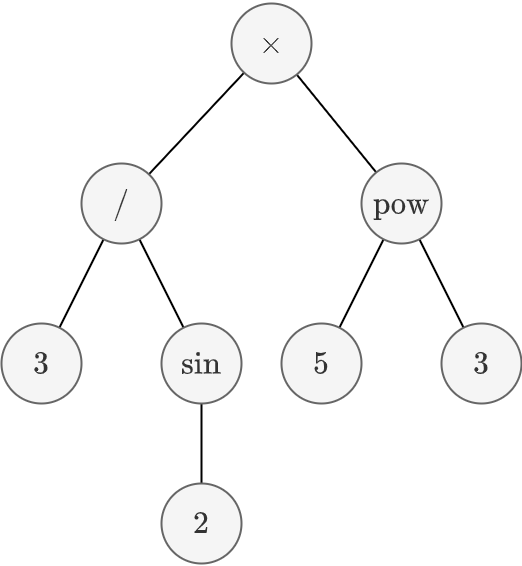
\includegraphics[height=5.5cm]{img/theoretical_framework/GP Initial Population 1.png}
      \caption{\(\mathbf{I}_1 = \mathlarger{\frac{3}{\sin(2)}} \times 5^3\)}
      \label{fig:genetic_programming:initialization:population:1}
    \end{subfigure}
    \begin{subfigure}[t]{0.4\textwidth}
      \centering
      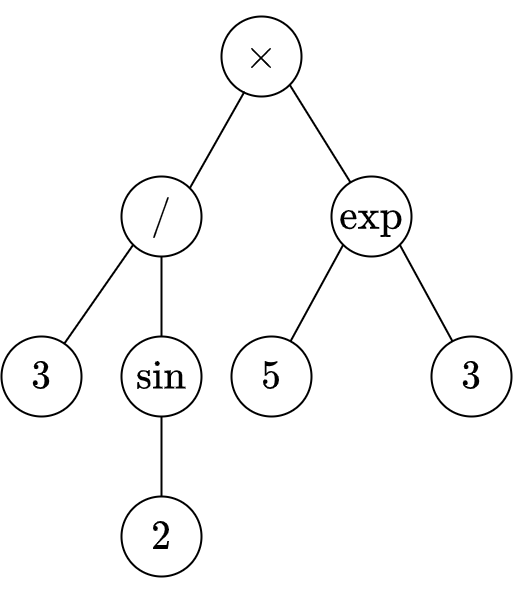
\includegraphics[height=5.5cm]{img/theoretical_framework/GP Initial Population 2.png}
      \caption{\(\mathbf{I}_2 = 7 - (5 + \sin(x))\)}
      \label{fig:genetic_programming:initialization:population:2}
    \end{subfigure}
    \begin{subfigure}[t]{0.4\textwidth}
      \centering
      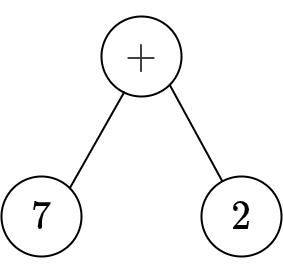
\includegraphics[height=2.75cm]{img/theoretical_framework/GP Initial Population 3.png}
      \caption{\(\mathbf{I}_3 = 7 + 2\)}
      \label{fig:genetic_programming:initialization:population:3}
    \end{subfigure}
    \begin{subfigure}[t]{0.4\textwidth}
      \centering
      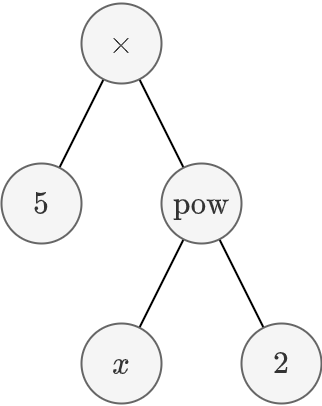
\includegraphics[height=4.125cm]{img/theoretical_framework/GP Initial Population 4.png}
      \caption{\(\mathbf{I}_4 = 5x^2\)}
      \label{fig:genetic_programming:initialization:population:4}
    \end{subfigure}
    \caption{A population of random trees.}
    \label{fig:genetic_programming:initialization:population}
  \end{figure}

  The next step is to calculate the fitness of each individual in the
  population.
  If we recall, the fitness function is the MSE between the expected output and
  the actual output of the individual.

  \begin{align*}
    \mathrm{MSE}(\mathbf{y}, \mathbf{I}_1[\mathbf{x}])
      & = \frac{1}{10} \sum_{i=1}^{10} (\mathbf{y}_i - \mathbf{I}_1(\mathbf{x}_i))^2
        = \frac{1}{10} \sum_{i=1}^{10} \left(
          \mathbf{y}_i - \frac{3}{\sin(2)} \cdot 5^3\right)^2 \\
      & \approx 177\,596.851\,131  \\
    \mathrm{MSE}(\mathbf{y}, \mathbf{I}_2[\mathbf{x}])
      & = \frac{1}{10} \sum_{i=1}^{10} (\mathbf{y}_i - \mathbf{I}_2(\mathbf{x}_i))^2
        = \frac{1}{10} \sum_{i=1}^{10} \left(
          \mathbf{y}_i - 7 - (5 + \sin(x_i))\right)^2 \\
      & \approx 137.398\,836  \\
    \mathrm{MSE}(\mathbf{y}, \mathbf{I}_3[\mathbf{x}])
      & = \frac{1}{10} \sum_{i=1}^{10} (\mathbf{y}_i - \mathbf{I}_3(\mathbf{x}_i))^2
        = \frac{1}{10} \sum_{i=1}^{10} \left(
          \mathbf{y}_i - (7 + 2)\right)^2 \\
      & \approx 331.924\,267 \\
    \mathrm{MSE}(\mathbf{y}, \mathbf{I}_4[\mathbf{x}])
      & = \frac{1}{10} \sum_{i=1}^{10} (\mathbf{y}_i - \mathbf{I}_4(\mathbf{x}_i))^2
        = \frac{1}{10} \sum_{i=1}^{10} \left(
          \mathbf{y}_i - 5x^2\right)^2 \\
      & \approx 138.079\,865
  \end{align*}

  With this, we can assign a fitness to each individual in the population as
  shown in \vref{tab:genetic_programming:initialization:population}.
  A summary of the population's fitness is shown in
  \vref{tab:genetic_programming:initialization:fitness}.

  \begin{table}[ht!]
    \centering
    \begin{tabular}{c|c|c|r}
      \multicolumn{4}{c}{\textbf{Generation 0}} \\
      \hline
      \hline
      \textbf{Individual} & \textbf{Program} & \textbf{Depth} & \textbf{Fitness} \\
      \hline
      \(\mathbf{I}_1\) 
        & \Gape[2pt][2pt]{\(\frac{3}{\sin(2)} \times 5^3 \)} & 3 & 177\,596.851\,131 \\
      \(\mathbf{I}_2\) & \Gape[2pt][2pt]{\(7 - (5 + \sin(x))\)} & 3 & 137.398\,836 \\
      \(\mathbf{I}_3\) & \Gape[2pt][2pt]{\(7 + 2\)} & 1 & 331.924\,267 \\
      \(\mathbf{I}_4\) & \Gape[2pt][2pt]{\(5x^2\)} & 2 & 138.079\,865
    \end{tabular}
    \caption{Population of individuals in generation 0}
    \label{tab:genetic_programming:initialization:population}
  \end{table}

  \begin{table}[ht!]
    \centering
    \begin{tabular}{|c|r|c|}
      \hline
      & \textbf{Fitness} & \textbf{Individual}  \\
      \hline
      Best & 137.398\,836 & \(\mathbf{I}_2\) \\
      Worst & 177\,596.851\,131 & \(\mathbf{I}_1\) \\
      \hline
      \hline
      Average & \multicolumn{2}{r|}{44\,551.063\,525} \\
      \hline
      Standard Deviation & \multicolumn{2}{r|}{88\,697.238\,974} \\
      \hline
    \end{tabular}
    \caption{Fitness of the individuals in generation 0}
    \label{tab:genetic_programming:initialization:fitness}
  \end{table}

  We can observe that the worst individual has an error significantly larger
  than the best individual.
  This is to be expected, as the MSE is a measure of the error that escalates
  exponentially with the difference between the expected and actual output.  

  A graphical representation of the population is shown in
  \vref{fig:genetic_programming:initialization:population_graph}.
  It is clear from the figure that the worst individual is \(\mathbf{I}_1\).

  \begin{figure}[ht!]
    \centering
    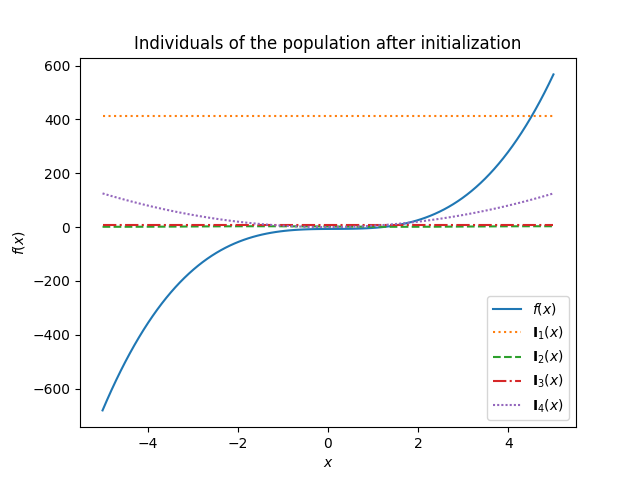
\includegraphics[width=0.6\textwidth]{img/theoretical_framework/gp_pop_init.png}
    \caption{
      Graphical representation of the population in generation 0 compared to the
      expected output.
    }
    \label{fig:genetic_programming:initialization:population_graph}
  \end{figure}

  
  In summary, the initialization stage of the genetic programming algorithm, a 
  population of random individuals, represented as trees, was generated using 
  the \enquote{grow method}.
  The height of these trees, signifying the length of the longest path from the
  root to a leaf, is determined randomly within a specified range.
  Each tree is recursively populated with random nodes until a terminal node is
  chosen or the maximum height is reached.
  Once a random population of trees is created, the fitness of each individual,
  based on the Mean Squared Error (MSE) between the expected and actual output,
  is calculated.
  This results in the assignment of fitness scores to all individuals,
  facilitating the evaluation and selection process in the succeeding stages of
  the algorithm.
  The output of this process is a random population of trees with fitness scores
  and height measurements, ready for the next steps of selection, crossover, and
  mutation.
